\documentclass[11pt, twosides]{article}
\usepackage[utf8]{inputenc}
\usepackage{graphicx}
\usepackage{graphics}
\usepackage{amsmath}
\usepackage{amsfonts}
\usepackage{amssymb}
\usepackage{amsthm}
\usepackage{cancel} % for \cancel
\usepackage{bbm} % for indicator functions
\usepackage{xcolor}
\setlength{\oddsidemargin}{0.25 in}
\setlength{\evensidemargin}{-0.25 in}
\setlength{\topmargin}{-0.6 in}
\setlength{\textwidth}{6.5 in}
\setlength{\textheight}{8.5 in}
\setlength{\headsep}{0.75 in}
\setlength{\parindent}{0 in}
\setlength{\parskip}{0.1 in}
\usepackage[section]{placeins}
\usepackage[section]{placeins}
\usepackage[section]{placeins}
\usepackage[section]{placeins}
\usepackage[section]{placeins}
\usepackage[section]{placeins}
\usepackage{float}
\usepackage{siunitx}
%
% The following commands set up the lecnum (lecture number)
% counter and make various numbering schemes work relative
% to the lecture number.
%
\newcounter{lecnum}
\renewcommand{\thepage}{\thelecnum-\arabic{page}}
\renewcommand{\thesection}{\thelecnum.\arabic{section}}
\renewcommand{\theequation}{\thelecnum.\arabic{equation}}
\renewcommand{\thefigure}{\thelecnum.\arabic{figure}}
\renewcommand{\thetable}{\thelecnum.\arabic{table}}

%
% The following macro is used to generate the header.
%
\newcommand{\lecture}[4]{
%   \pagestyle{myheadings}
   \thispagestyle{plain}
   \newpage
   \setcounter{lecnum}{#1}
   \setcounter{page}{1}
   \noindent
   \begin{center}
   \framebox{
      \vbox{\vspace{2mm}
    \hbox to 6.28in { {\bf CS 419M Introduction to Machine Learning
                        \hfill Spring 2021-22} }
       \vspace{4mm}
       \hbox to 6.28in { {\Large \hfill Lecture #1: #2  \hfill} }
       \vspace{2mm}
       \hbox to 6.28in { {\it Lecturer: #3 \hfill Scribe: #4} }
      \vspace{2mm}}
   }
   \end{center}
   \markboth{Lecture #1: #2}{Lecture #1: #2}
}

%
% Convention for citations is authors' initials followed by the year.
% For example, to cite a paper by Leighton and Maggs you would type
% \cite{LM89}, and to cite a paper by Strassen you would type \cite{S69}.
% (To avoid bibliography problems, for now we redefine the \cite command.)
% Also commands that create a suitable format for the reference list.
% \renewcommand{\cite}[1]{[#1]}
% \def\beginrefs{\begin{list}%
%         {[\arabic{equation}]}{\usecounter{equation}
%          \setlength{\leftmargin}{2.0truecm}\setlength{\labelsep}{0.4truecm}%
%          \setlength{\labelwidth}{1.6truecm}}}
% \def\endrefs{\end{list}}
% \def\bibentry#1{\item[\hbox{[#1]}]}

%Use this command for a figure; it puts a figure in wherever you want it.
%usage: \fig{NUMBER}{SPACE-IN-INCHES}{CAPTION}
% \newcommand{\fig}[3]{
% 			\vspace{#2}
% 			\begin{center}
% 			Figure \thelecnum.#1:~#3
% 			\end{center}
% 	}
% Use these for theorems, lemmas, proofs, etc.
\newtheorem{theorem}{Theorem}[lecnum]
\newtheorem{lemma}[theorem]{Lemma}
\newtheorem{proposition}[theorem]{Proposition}
\newtheorem{claim}[theorem]{Claim}
\newtheorem{corollary}[theorem]{Corollary}
\newtheorem{definition}[theorem]{Definition}
% \newenvironment{proof}{{\bf Proof:}}{\hfill\rule{2mm}{2mm}}

% ** IF YOU WANT TO DEFINE ADDITIONAL MACROS FOR YOURSELF, PUT THEM HERE:

\begin{document}
%FILL IN THE RIGHT INFO.
%\lecture{*LECTURE-NUMBER}{DATE}{LECTURER}{SCRIBE*}
\lecture{18}{Convolution Function and Activation Map}{Abir De}{Group2}
%\lecture{x}{Title}{Abir De}{Group y}

\section{Convolution Operation}

\textbf{Neuron} 
  \\
  3 x 3 (input) $-> z ->$ activation(z)
  
  \\
  $z_1 = w_0 +w_1x_1 + w_2x_2 + w_3x_3 + w_4x_6 + w_5x_7 + w_6x_8 + w_7x11 + w_8x_12 + w_9x_13$

Now, the filter will select a subset 3 x 3 matrix 


\begin{figure}[H]
\centering
\caption{Convolution Operation}
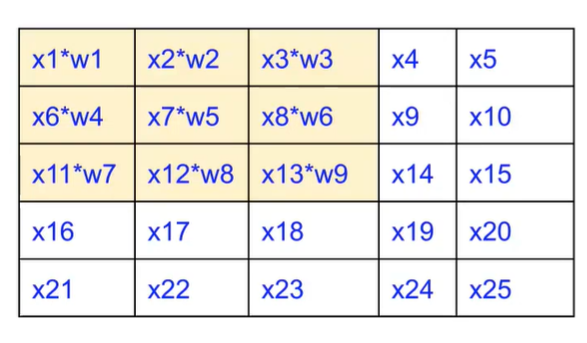
\includegraphics[scale = 0.5]{419sc1.png}
\end{figure}
 %\FloatBarrier

$O_1 = Output_1 = g(z) = ReLu(z)$\\
 
Now, shift by one column to right and compute z2 in a similar manner\\
$z_2 = w_0 + w_1x_2 + w_2x_3 + w_3x_4 + w_4x_7 + w_5x_8 + w_6x_9 + w_7x12 + w_8x_13 + w_9x_14$

\begin{figure}[H]
\centering
\caption{Convolution Operation}
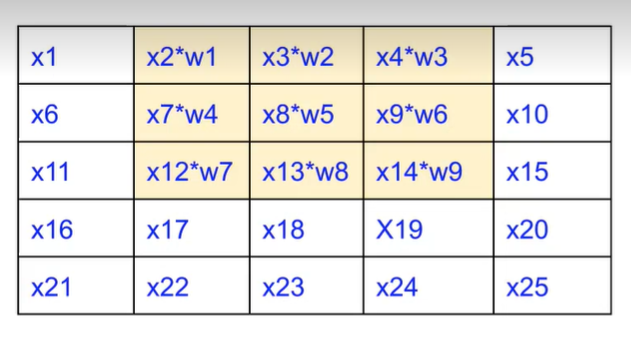
\includegraphics[scale = 0.5]{419sc2.png}
\end{figure}
\\
$O_2 = Output_2 = g(z) = ReLu(z)$\\
\\
Now, shift by one more column to right and compute z3 in a similar manner\\
$O_3 = Output_3 = g(z) = ReLu(z)$\\

\textbf{Activation Map}
\\

\begin{table}[!hbt]
	\begin{center}
	\caption{Filter 1\\}
	\begin{tabular}{|c|c|c|}
		\hline
        $O_1$ & $O_2$ & $O_3$\\
		\hline
        $O_4$ & $O_5$ & $O_6$\\
		\hline
        $O_7$ & $O_8$ & $O_9$\\
		\hline
	\end{tabular}
	\end{center}
\end{table}
In similar manner, we will get activation map from different filters.\\

Each filter is representing a neural operation\\
\begin{figure}[H]
\centering
\caption{Convolution Operation}
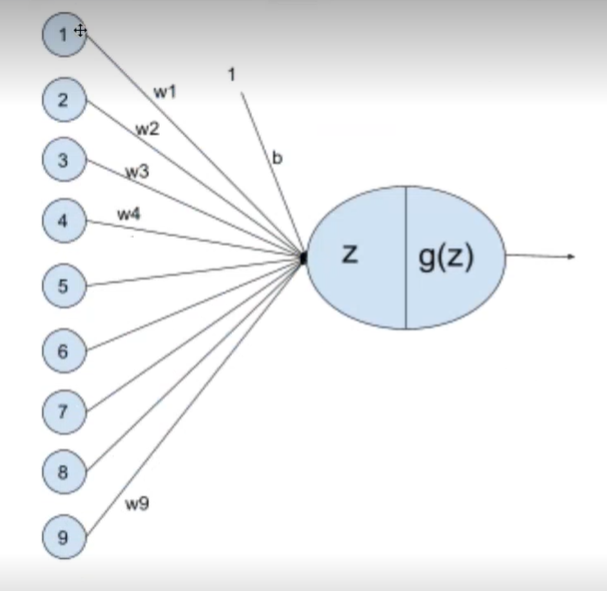
\includegraphics[scale = 0.6]{419sc3.png}
\end{figure}
\\
\textbf{How does convolution happen in 3D image?}
\\ 
3D filter is used for convolution of 3D image\\

$3D filter -> $ 3 x 3 x 3 

\\
The number of channels in a filter is not defined by default. It is implicit. It is equal to the number of channels in the input
\newpage

% Suggested surrogate function is $exp(-w^T x)$. In order to minimize the sum of this function over w
% \begin{itemize}
%     \item If $w^T x >$ 1 then y = 1
%     \item If $w^T x <$ -1 then y = -1
% \end{itemize}
% One suitable surrogate function is the hinge function, defined as :
% \begin{itemize}
%     \item y = 1 and  $w^T x >$ 1 then loss = 0
%     \item y = -1 and  $w^T x <$ 1 then loss = 0

% \end{itemize}
%  Loss($w^Tx$, y) = max(0 , 1-$w^Tx$y)
 
% Our loss functions approximate to \sum_{x,y\in\ D}I(h(x) $\not=$ y) in some sense

% Hinge function is also given as :
% $(1-$w^Tx$y)_+$ = ReLU(1-$w^Tx$y)


% \textbf{Probabilistic Approach} :
% For the same problem we can also use a probabilistic approach, Suppose X is sampled from a probability distribution and Y is sampled from a probability distribution conditioned on x.

% Now, we try to estimate \sum_{x,y\in\ D}I(h(x) $\not=$ y) in terms of probability.

% Using, Law of large numbers

% [\sum_{x,y\in\ D}I(h(x) $\not=$ y)]/$|D|$ \approx E[I(h(x) $\not=$ y)]] = P(h(x) $\not=$ y)
% \begin{enumerate}
%     \item Conditional Independence or probabilities, Bayesian relationship
%     \item Introducing Random Variables: Bernoulli, Normal, Poisson
%     \item Expectation, Variance, Covariance
%     \item Central Limit Theorem, Law of large numbers
% \end{enumerate}

% \subsection{Why Probability is important for Machine Learning?}
% Suppose you have a set of \textbf{Data}. This can be
% \begin{itemize}
%     \item A set of images $\xrightarrow{m_\theta}$ identify the objects
%     \item A set of paragraphs $\xrightarrow{m_\theta}$ identify the topics 
% \end{itemize}
% where $m_\theta$ denotes a model with parameters $\theta$. The objective is to devise a model which learns to do a task. The following question can be posed:
% \begin{flushleft}
% Q. \textbf{What is the underlying thesis/concept behind the hope that it will be possible to train the model $m_\theta$ to get an accurate output?}\\

% Ans. \color{blue}
% \textbf{The law of large numbers}
% \end{flushleft}

% \subsection{The Law of Large Numbers and Central Limit Theorem}
% Suppose that we have $N$ samples $X_i \sim f(\cdot), \:\:\: i = 1, \hdots, N$ drawn from an unknown distribution. Most of the times, the goal of machine learning is to estimate the distribution $f$ or its properties. For example, in the task of generating images (GAN, VAE etc), the objective of the machine learning model is to identify the underlying distribution of the data samples. Being able to learn the underlying distribution is important even for tasks like housing price prediction, image classification etc because if a test sample is sampled from a different distribution is given to the model, the model will likely fail and give incorrect results. 
% \begin{flushleft}
% Q. \textbf{What is the least that can be found about $f$ using $X_1, \hdots, X_N$?}\\

% Ans. \color{blue} Central Limit Theorem states that as long as $N$ is large, the $$\mathbb{E}_{X \sim f(\cdot)}[X] = \frac{\sum X_i}{N}$$
% The Law of Large Numbers further states that
% $$\mathbb{E}_{X \sim f(\cdot)}[X] \xrightarrow{}\frac{\sum X_i}{N}$$
% as $N \xrightarrow{} \infty$. Moreover, the random variable $Z_N = \frac{\sum X_i}{N}$ follows the normal distribution $\mathcal{N}(\mathbb{E}[X], \sigma^2)$
% with $\sigma^2 \propto \frac{1}{N}$ with
% $$\lim \limits_{N \xrightarrow{}\infty}\mathbb{E}[Z_N] = \mathbb{E}[X]$$
% \end{flushleft}
% \begin{flushleft}
% Q. \textbf{What else do we need to completely characterize $f$?}\\

% Ans. \color{blue} \textbf{We need the higher order moments!} Using these the moment generating function can be obtained.
% \end{flushleft}

% \definition{The moment generating function (MGF) $F(s)$ for a random variable $X$ is defined as the Laplace Transform of the probability density function (PDF) $f(x)$. The inverse Laplace Transform of MGF will give the PDF.
% $$F(s) = \int \limits_{-\infty}^\infty e^{-sx}\, f(x)\, dx$$
% $$f(x) = \int \limits_{-\infty}^\infty e^{sx}\, F(s)\, ds$$}

% \proposition{Using only the moments, the MGF can be determined.}
% \begin{proof}
% \begin{eqnarray*}
% F(s) &=& \int \limits_{-\infty}^\infty e^{-sx}\, f(x)\, dx\\
% &=& \int \limits_{-\infty}^\infty \sum \limits_{k = 0}^{\infty} \frac{(-s)^k\, x^k}{k!}\, f(x)\, dx\\
% &=& \sum \limits_{k = 0}^{\infty} \frac{(-s)^k}{k!}\, \mathbb{E}[X^k]
% \end{eqnarray*}
% \begin{flushleft}
% Note: The discussion about the region of convergence of the Laplace transform is out of the scope of this course.
% \end{flushleft}
% \end{proof}

% \proposition{
% Using just the $N$ samples $X_i \sim f(\cdot), \:\:\: i = 1, \hdots, N$, the PDF $f$ can be estimated using the Law of Large Numbers.
% }
% \begin{proof}
% This can be proved as follows:
% \begin{enumerate}
%     \item All moments $\mathbb{E}[X^k]$ can be estimated by invoking the Law of Large Numbers
%     \item The MGF can be found by invoking the Claim 1.2 above.
%     \item $f$ can be estimated by taking the inverse Laplace Transform of the MGF
% \end{enumerate}
% \end{proof}

% \subsection{Practice Problems}
% \normalfont
% \begin{enumerate}
%     \item  A fair coin is tossed 5 times. Find  $\mathbb{P}(\#H > \# T)$\\
%     \color{blue}It is easy to see that as 5 is odd, there is not possibility of $\#H = \#T$. Hence $\mathbb{P}(\#H > \# T) = 1/2$
%     \color{black}
%     \item $X \sim f(\cdot), Y \sim g(\cdot)$. Then $Z = X+Y \sim \:?$\\
%     \color{blue} \begin{eqnarray*}
%     \mathbb{P}(Z \leq z) &=& \mathbb{P}(X+Y \leq z)\\
%                         &=& \int \limits_{-\infty}^\infty \int \limits_{-\infty}^{z-x}f(x) \, g(y) \, dx\,dy\\
%                         &=& \int \limits_{-\infty}^\infty f(x)\, G(z-x) \, dx
%     \end{eqnarray*}
%     On differentiating, we get
%     $$f_Z(z) = \int \limits_{-\infty}^\infty f(x) g(z-x)\,dx = (f * g)(z)$$
% \end{enumerate}
% \section{Linear Algebra}
% Solve the following problems:
% \begin{enumerate}
%     \item For two square matrices $A, B$of size $n\times n$ if $AB = BA$ for all B, then show that $A = cI_n$ for some $c \in \mathbb{R}$\\
%     \color{blue}
%     Pick $B$ to be a diagonal matrix with pair-wise distinct elements. Then it can be shown that $A$ is also a diagonal matrix. Now pick $B$ to be a matrix with all ones, i.e. $B = [1]_{ij}$. As $A$ is diagonal, $AB=BA$ implies all diagonal entries of $A$ are equal i.e., $A = cI_n$ for some $c \in \mathbb{R}$
%     \color{black}
%     \item If $x^\top A x = 0\:\: \forall x \in \mathbb{R}^n$ then show that $A$ is skew-symmetric.\\
%     \color{blue}
%     On differentiating the above equation we get
%     $$(A + A^\top)x = 0 \:\: \forall x \in \mathbb{R}^n$$
%     This implies $A = -A^\top$
%     \color{black}
%     \item Show that $\text{rank}(AB) \leq \text{rank}(A)$\\
%     \color{blue} Each column of $AB$ can be viewed as a linear combination of columns of $A$. Hence, if the dimension of column space of $A$ is $r$, the dimension of column space of $AB$ cannot be more than $r$. In other words,
%     $\text{rank}(AB) \leq \text{rank}(A)$
%     \color{black}
%     \item Suppose you have a uniform sampler which samples uniformly from $[0, 1]$. Propose an algorithm which uses this uniform sampler to generate samples from any given distribution.\\
%     \color{blue}
%     Suppose we have a uniform random variable $U \sim \text{Uniform}([0, 1])$. We need to find a function $g$ such that the PDF of the random variable $g(U)$ will be same as that of the given distribution, say $f$. That is $g(U) \sim f$. Which is same as
%     \begin{eqnarray*}
%     \mathbb{P}(g(U) \leq x) &=& \mathbb{P}(U \leq g^{-1}(x))\\
%     \implies \int \limits_{-\infty}^x f(x) \, dx &=& \int \limits_{-\infty}^{g^{-1}(x)} 1 \, du\\
%     \implies F(x) &=& g^{-1}(x)\\
%     \implies g &=& F^{-1}
%     \end{eqnarray*}
%     \color{black}
% \end{enumerate}
\section{Group Details and Individual Contribution}
% Fill this part
\item Prakriti Shetty, 200020095: Contributed to Convolution Operation- Neuron writeup
\item Shirish Chinchanikar, 19B090012: Contributed to Convolution Operation- Activation Map writeup
\item Yuvraj Singh, 200070093: Contributed to Convolution Operation- Neuron writeup
\item Neeraj Patidar, 19D070039: Contributed to Convolution Operation- Neuron writeup
\item Saeel Nachane, 20D180028: Contributed to Convolution Operation- Activation Map writeup
\end{document}
